\documentclass{beamer}
\usepackage[english, russian]{babel}
\usepackage[T2A]{fontenc}
\usepackage[utf8]{inputenc}
\usepackage{indentfirst}
\usepackage{amsmath, amsfonts, amssymb, amsthm, mathtools}
\usepackage[export]{adjustbox}
\usepackage{graphicx} 
\graphicspath{ {./images/} }

\usepackage{subcaption}
\usepackage{verbatim}

\usepackage{minted}{\setlength{\parskip}{0pt}}

\usepackage{hyperref}

\hypersetup{
    colorlinks=true,
    linkcolor=blue,
    filecolor=magenta,      
    urlcolor=black,
    pdftitle={Overleaf Example},
    pdfpagemode=FullScreen,
    }


\title{Отчет по лабораторной работе № 4. \\ Базовая настройка HTTP-сервера Apache}
\author{Данила Стариков \\ НПИбд-02-22}
\date{2024}

\begin{document}

\maketitle
\newpage

\tableofcontents

\newpage
\section{Цель работы}
Приобретение практических навыков по установке и базовому конфигурированию HTTP-сервера Apache.
\newpage
\section{Выполнение работы}

\subsection{Установка HTTP-сервера}
\begin{enumerate}

\item Загрузили вашу операционную систему и перешли в рабочий каталог с проектом:
\begin{minted}{bash}
 cd /var/tmp/dastarikov/vagrant
\end{minted}

\item Запустили виртуальную машину {\t server}:
\begin{minted}{bash}
make server-up
\end{minted}
\item На виртуальной машине server вошли и открыли терминал. Перешли в режим суперпользователя.
\item Установили из репозитория стандартный веб-сервер (HTTP-сервер и утилиты httpd, криптоутилиты и пр.):
\begin{minted}{bash}
LANG=C yum grouplist
dnf -y groupinstall "Basic Web Server"
\end{minted}
\end{enumerate}

\subsection{Базовое конфигурирование HTTP-сервера}
\begin{enumerate}
\item Просмотрели и прокомментировали в отчёте содержание конфигурационных файлов в каталогах {\tt /etc/httpd/conf} и {\tt /etc/httpd/conf.d}.
\item Внесли изменения в настройки межсетевого экрана узла server, разрешив работу с http (Рис. \ref{01}):
\begin{minted}{bash}
firewall-cmd --list-services
firewall-cmd --get-services
firewall-cmd --add-service=http
firewall-cmd --add-service=http --permanent
\end{minted}

\begin{center}
    \centering
    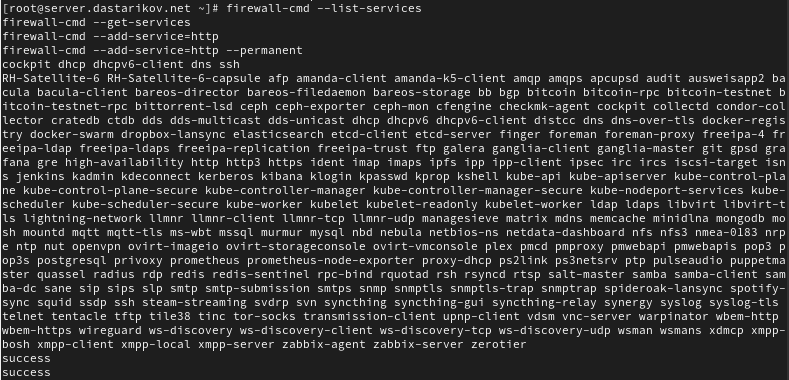
\includegraphics[width=0.9\textwidth]{../images/image01.png}
    \captionof{figure}{Настройка межсетевого экрана.}
    \label{01}
\end{center}

\item В дополнительном терминале запустили в режиме реального времени расширенный лог системных сообщений, чтобы проверить корректность работы системы (Рис. \ref{02}):

\begin{minted}{bash}
journalctl -x -f
\end{minted}
\item В первом терминале активировали и запустили HTTP-сервер:
\begin{minted}{bash}
systemctl enable httpd
systemctl start httpd
\end{minted}

\begin{center}
    \centering
    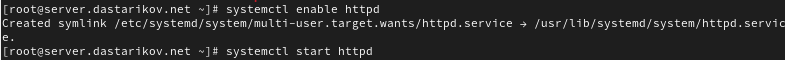
\includegraphics[width=0.9\textwidth]{../images/image02.png}
    \captionof{figure}{Запуск HTTP-сервера.}
    \label{02}
\end{center}

Просмотрев расширенный лог системных сообщений, убедились, что веб-сервер успешно запустился.
\end{enumerate}

\subsection{Анализ работы HTTP-сервера}
\begin{enumerate}

\item Запустили виртуальную машину client:
\begin{minted}{bash}
make client-up
\end{minted}

\item На виртуальной машине server просмотрели лог ошибок работы веб-сервера:
\begin{minted}{bash}
tail -f /var/log/httpd/error_log
\end{minted}
\item На виртуальной машине server запустили мониторинг доступа к веб-серверу:
\begin{minted}{bash}
tail -f /var/log/httpd/access_log
\end{minted}
На виртуальной машине client запустили браузер и в адресной строке ввели 192.168.1.1 (Рис. \ref{03} и  \ref{14}).


\begin{center}
    \centering
    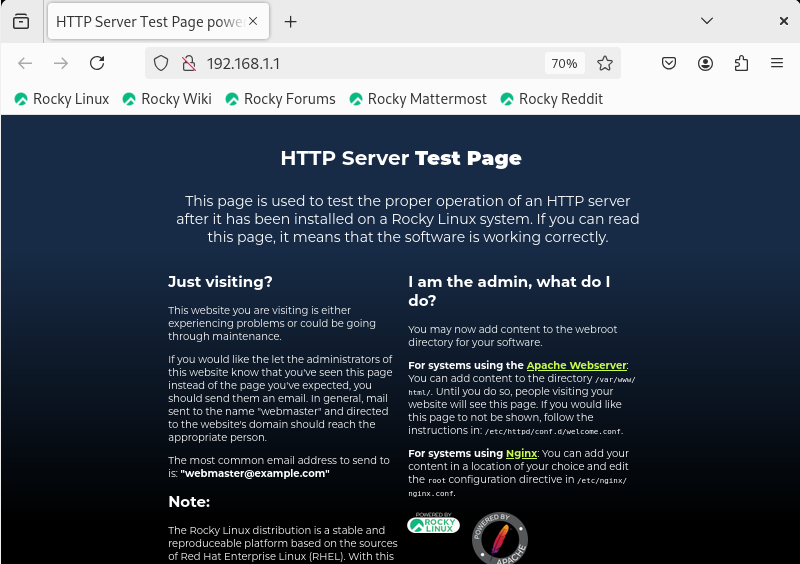
\includegraphics[width=0.9\textwidth]{../images/image03.png}
    \captionof{figure}{Запуск тестовой страницы.}
    \label{03}
\end{center}

\begin{center}
    \centering
    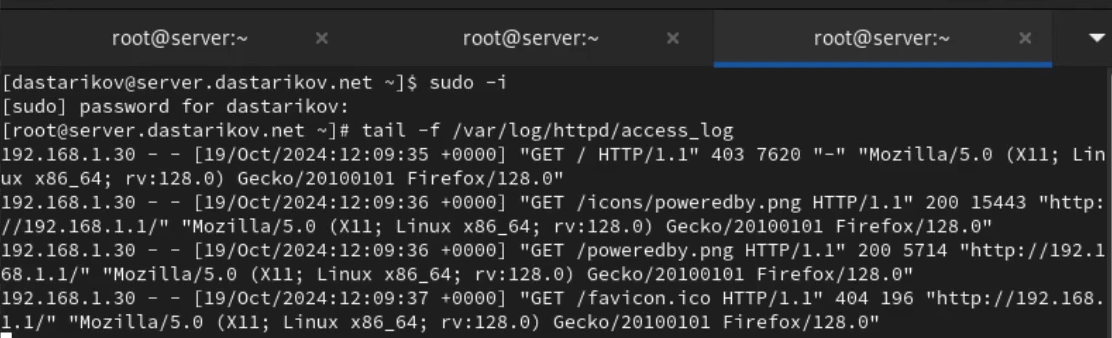
\includegraphics[width=0.9\textwidth]{../images/image14.png}
    \captionof{figure}{Записи в журнале мониторинга доступка к веб-серверу}
    \label{14}
\end{center}

\end{enumerate}

\subsection{Настройка виртуального хостинга для HTTP-сервера}
Требуется настроить виртуальный хостинг по двум DNS-адресам: server.dastarikov.net и www.dastarikov.net.
\begin{enumerate}
\item Остановили работу DNS-сервера для внесения изменений в файлы описания DNS-зон:
\begin{minted}{bash}
systemctl stop named
\end{minted}
\item Добавили запись для HTTP-сервера в конце файла прямой DNS-зоны \break \texttt{/var/named/master/fz/dastarikov.net} (Рис. \ref{05}):
\begin{minted}{bash}
www A 192.168.1.1
\end{minted}

\begin{center}
    \centering
    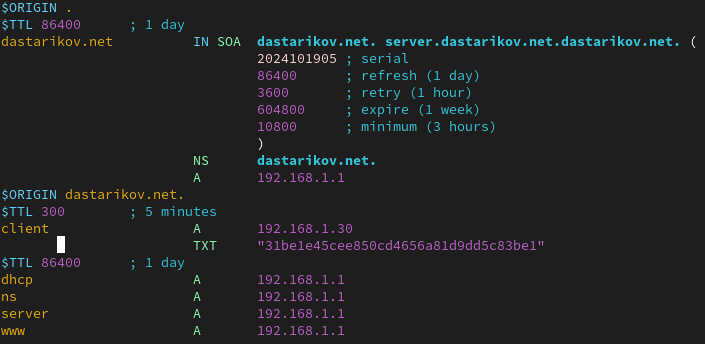
\includegraphics[width=0.9\textwidth]{../images/image05.png}
    \captionof{figure}{Обновление файла прямой DNS-зоны.}
    \label{05}
\end{center}

и в конце файла обратной зоны \texttt{/var/named/master/rz/192.168.1} (Рис. \ref{07}):
\begin{minted}{bash}
1 PTR www.dastarikov.net.
\end{minted}

\begin{center}
    \centering
    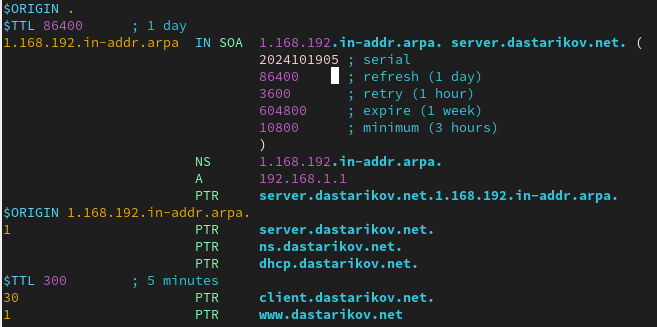
\includegraphics[width=0.9\textwidth]{../images/image07.png}
    \captionof{figure}{Обновление файла обратной DNS-зоны.}
    \label{07}
\end{center}

% Вместо dastarikov укажите свой логин. При этом не забудьте из соответствующих каталогов удалить файлы журналов DNS: dastarikov.net.jnl и 192.168.1.jnl.
\item Перезапустили DNS-сервер:
\begin{minted}{bash}
systemctl start named
\end{minted}
\item В каталоге \texttt{/etc/httpd/conf.d} создали файлы \texttt{server.dastarikov.net.conf} и \break \texttt{www.dastarikov.net.conf}:
\begin{minted}{bash}
cd /etc/httpd/conf.d
touch server.dastarikov.net.conf
touch www.dastarikov.net.conf
\end{minted}
\item Открыли на редактирование файл \texttt{server.dastarikov.net.conf} и внесли следующее содержание (Рис. \ref{08}):
\begin{minted}{bash}
<VirtualHost *:80>
ServerAdmin webmaster@dastarikov.net
DocumentRoot /var/www/html/server.dastarikov.net
ServerName server.dastarikov.net
ErrorLog logs/server.dastarikov.net-error_log
CustomLog logs/server.dastarikov.net-access_log common
</VirtualHost>
\end{minted}

\begin{center}
    \centering
    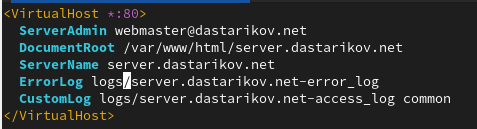
\includegraphics[width=0.9\textwidth]{../images/image08.png}
    \captionof{figure}{Изменение server.dastarikov.net.conf.}
    \label{08}
\end{center}

\item Открыли на редактирование файл {\tt www.dastarikov.net.conf} и внесли следующее содержание (Рис. \ref{09}):
\begin{minted}{bash}
<VirtualHost *:80>
ServerAdmin webmaster@dastarikov.net
DocumentRoot /var/www/html/www.dastarikov.net
ServerName www.dastarikov.net
ErrorLog logs/www.dastarikov.net-error_log
CustomLog logs/www.dastarikov.net-access_log common
</VirtualHost>
\end{minted}

\begin{center}
    \centering
    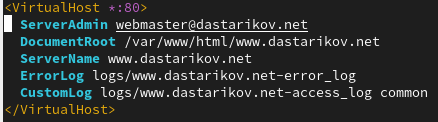
\includegraphics[width=0.9\textwidth]{../images/image09.png}
    \captionof{figure}{Изменение www.dastarikov.net.conf.}
    \label{09}
\end{center}

\item Перешли в каталог {\tt /var/www/html}, в котором должны находиться файлы с содержимым (контентом) веб-серверов, и создали тестовые страницы для виртуальных веб-серверов {\tt server.dastarikov.net} и {\tt www.dastarikov.net}.
Для виртуального веб-сервера {\tt server.dastarikov.net}:
\begin{minted}{bash}
cd /var/www/html
mkdir server.dastarikov.net
cd /var/www/html/server.dastarikov.net
touch index.html
\end{minted}
Открыли на редактирование файл {\tt index.html} и внесли следующее содержание:
\begin{minted}{bash}
Welcome to the server.dastarikov.net server.
\end{minted}
Для виртуального веб-сервера {\tt www.dastarikov.net}:
\begin{minted}{bash}
cd /var/www/html
mkdir www.dastarikov.net
cd /var/www/html/www.dastarikov.net
touch index.html
\end{minted}

Открыли на редактирование файл {\tt index.html} и внесли следующее содержание
\begin{minted}{bash}
Welcome to the www.dastarikov.net server.
\end{minted}

\item Скорректировали права доступа в каталог с веб-контентом:
\begin{minted}{bash}
chown -R apache:apache /var/www
\end{minted}
\item Восстановили контекст безопасности в SELinux (Рис. \ref{10}):
\begin{minted}{bash}
restorecon -vR /etc
restorecon -vR /var/named
restorecon -vR /var/www
\end{minted}

\begin{center}
    \centering
    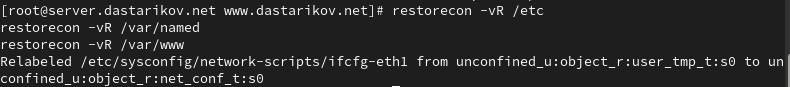
\includegraphics[width=0.9\textwidth]{../images/image10.png}
    \captionof{figure}{Восстановление контекста безопасности SELinux.}
    \label{10}
\end{center}

\item Перезапустили HTTP-сервер:
\begin{minted}{bash}
systemctl restart httpd
\end{minted}
\item На виртуальной машине client убедились в корректном доступе к веб-серверу по адресам {\tt server.dastarikov.net} и {\tt www.dastarikov.net} в адресной строке веб-браузера (Рис. \ref{11} и \ref{12}).

\begin{center}
    \centering
    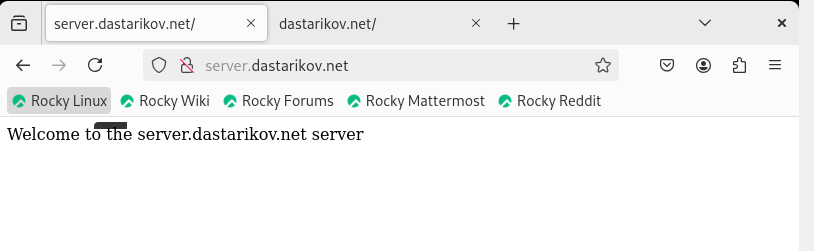
\includegraphics[width=0.9\textwidth]{../images/image11.png}
    \captionof{figure}{Проверка доступа к server.dastarikov.net.}
    \label{11}
\end{center}

\begin{center}
    \centering
    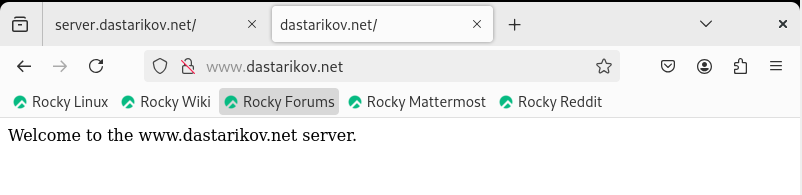
\includegraphics[width=0.9\textwidth]{../images/image12.png}
    \captionof{figure}{Проверка доступа к www.dastarikov.net.}
    \label{12}
\end{center}
\end{enumerate}      

\subsection{Внесение изменений в настройки внутреннего окружения виртуальной машины}
\begin{enumerate}
\item На виртуальной машине server перешли в каталог для внесения изменений в настройки внутреннего окружения {\tt /vagrant/provision/server/}, создали в нём каталог http, в который поместили в соответствующие подкаталоги конфигурационные файлы HTTP-сервера:
\begin{minted}{bash}
cd /vagrant/provision/server
mkdir -p /vagrant/provision/server/http/etc/httpd/conf.d
mkdir -p /vagrant/provision/server/http/var/www/html
cp -R /etc/httpd/conf.d/* /vagrant/provision/server/http/etc/httpd/conf.d/
cp -R /var/www/html/* /vagrant/provision/server/http/var/www/html
\end{minted}
\item Заменили конфигурационные файлы DNS-сервера:
\begin{minted}{bash}
cd /vagrant/provision/server/dns/
cp -R /var/named/* /vagrant/provision/server/dns/var/named/
\end{minted}

\item В каталоге {\tt /vagrant/provision/server} создали исполняемый файл http.sh:
\begin{minted}{bash}
cd /vagrant/provision/server
touch http.sh
chmod +x http.sh
\end{minted}
Открыв его на редактирование, прописали в нём следующий скрипт:
\begin{minted}{bash}
#!/bin/bash
echo "Provisioning script $0"
echo "Install needed packages"
dnf -y groupinstall "Basic Web Server"
echo "Copy configuration files"
cp -R /vagrant/provision/server/http/etc/httpd/* /etc/httpd
cp -R /vagrant/provision/server/http/var/www/* /var/www
chown -R apache:apache /var/www
restorecon -vR /etc
restorecon -vR /var/www
echo "Configure firewall"
firewall-cmd --add-service=http
firewall-cmd --add-service=http --permanent
echo "Start http service"
systemctl enable httpd
systemctl start httpd
\end{minted}
Этот скрипт, по сути, повторяет произведённые действия по установке и настройке HTTP-сервера.

\item Для отработки созданного скрипта во время загрузки виртуальных машин в конфигурационном файле Vagrantfile добавили в конфигурации сервера следующую запись:

\begin{minted}{bash}
server.vm.provision "server http",
type: "shell",
preserve_order: true,
path: "provision/server/http.sh"
\end{minted}
\end{enumerate}

\section{Выводы}
В результате выполнения лабораторной работы получили навыки по установке и базовому конфигурированию HTTP-сервера Apache.
\end{document}
